 \subsubsection{Estimaci\'on de la Tasa de Descuento Ke.}

Cuanto mayor sea el riesgo sistem\'atico de una acci\'on, m\'as elevado ser\'a el rendimiento que los inversionistas esperar\'an de los t\'itulos accionarios. Con la finalidad de estimar una tasa de descuento apropiada en pesos, en t\'erminos nominales y despu\'es de impuestos, se utilizaron los siguientes insumos para determinar el valor de la \gls{wacc}:\\


\textcolor{principal}{Tasa libre de riesgo (Rf).} Se basa en el rendimiento de los bonos gubernamentales, en este caso, se tom\'o en cuenta el pronóstico del rendimiento del \textcolor{principal}{\rfBase}, con el siguiente resultado:

\begin{figure}[H]
\centering
La tasa libre de riesgo obtenida es de \textbf{\rfValor\%}\\[10pt]
 \includegraphics[width=9cm]{\rutaImagenes/banxico/cuadro_1_jul-ago_2023}
\end{figure}

\gls{beta}. Con la finalidad de determinar el factor \gls{beta} apropiado para el negocio, se consider\'o una muestra de mercado de \glspl{leveredbeta} de empresas comparables al negocio valuado:

\textcolor{principal}{Muestra de mercado de la beta del sector,  estructura de Deuda/Capital del sector (D/E), tasa efectiva de impuestos a la utilidad (ETR\%) :}

\espacio{4cm}
\begin{figure}[H]
\centering
\includegraphics[width=6cm]{../0.imagenes/beta_1}\\
\end{figure}

La beta apalancada de sector que corresponde a la empresa es de \textcolor{principal}{\textbf{\valorBeta x }(mediana)}\\

F\'ormula de BETA Despalancada:
\begin{figure}[H]
\centering

\includegraphics[width=8cm]{\rutaImagenes/beta_apalancada}
\end{figure}

El valuador llev\'o a cabo la estimaci\'on del pron\'ostico de BETA desapalancada al negocio, habiendo aplicado a la proporci\'on de deuda/capital del sujeto, el promedio de la muestra y la tasa fiscal efectiva del sector (ETR\footnote{Efective Tax Rate}); con un resultado de \textcolor{principal}{\betaDesapalancada x}.\\

F\'ormula de BETA Reapalancada:\\

\begin{figure}[H]
\centering

\includegraphics[width=8cm]{\rutaImagenes/beta_reapalancada}
\end{figure}

Una vez obtenido el indicador de BETA desapalancada del sector, el valuador llev\'o a cabo la estimaci\'on del pron\'ostico de BETA reapalancada al negocio sujeto de valuaci\'on, habiendo aplicado a la proporci\'on de deuda/capital del sujeto, la mediana\footnote{Conforme a la aplicaci\'on del rango intercuartil como medida de estandarizaci\'on}  de la muestra del sector y la tasa fiscal de M\'exico (MTR\footnote{Marginal Tax Rate}), con un resultado de \textcolor{principal}{\betaReapalancada x}\\



\textcolor{principal}{Prima de riesgo del mercado de capitales}. Se obtuvo del promedio hist\'orico de la diferencia de rendimientos o ``\textit{spread}'' entre el mercado accionario \mercadoAccionario{} mediante el indicador conocido como el \gls{erp} (\textit{enterprise risk premium}).\\

\begin{figure}[H]
\centering
La prima de riesgo de mercado (\gls{erp}) es de \textbf{\textcolor{principal}{\erpValor\%}} \\[10pt]

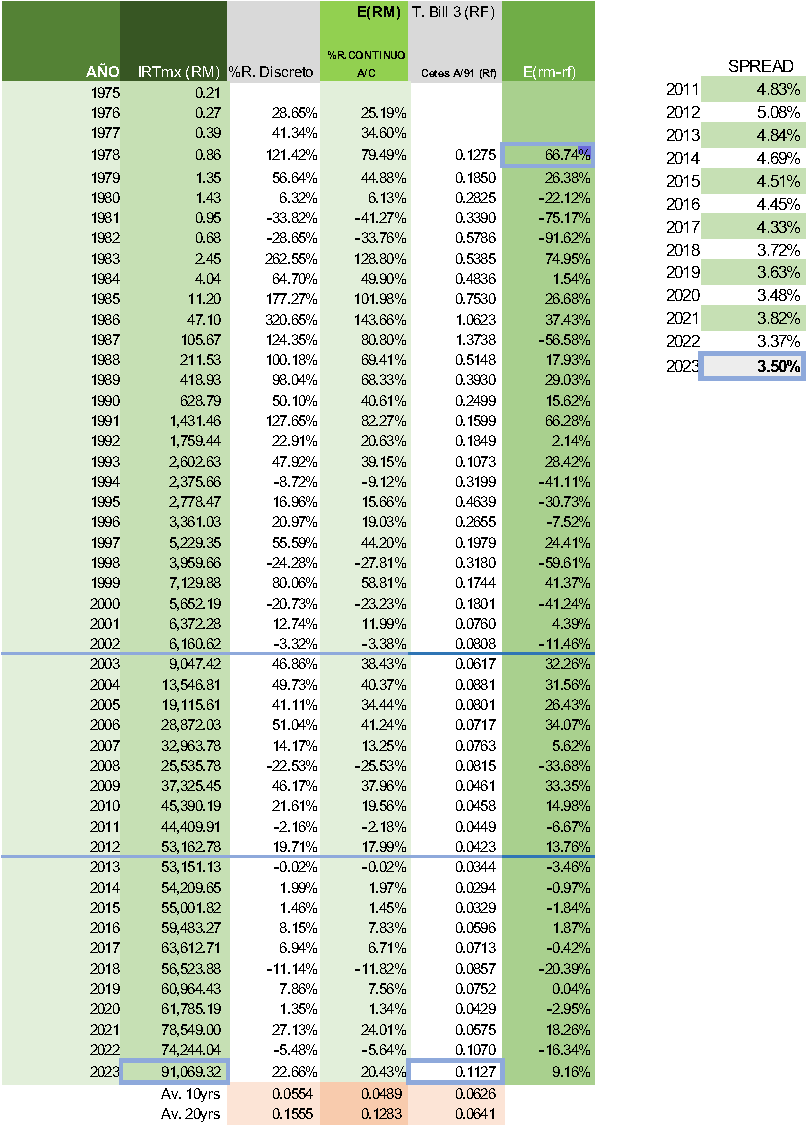
\includegraphics[width=5cm]{../0.imagenes/erp}
\end{figure}

%\textcolor{principal}{Riesgo Pa\'is (\gls{crp}).} Corresponde al riesgo pa\'is de M\'exico, seg\'un indicador de JP Morgan. Se considera un pron\'ostico para la prima de riesgo adicional de \crpValor{} puntos base.
%
%\begin{figure}[H]
%\centering
%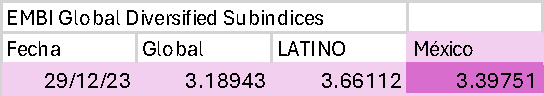
\includegraphics[width=8cm]{../0.imagenes/crp}
%\end{figure}

\textcolor{principal}{Prima por tamaño (\textit{Size Prime}).} \\[5pt]

Se tomo una prima por tamaño para la firma, a partir del valor en libros del capital contable de acuerdo a la siguiente tabla.\\

\textit{Nota. La tabla muestra la prima por tamaño a partir del valor en libros del capital contable en Millones de Euros.% Considerando el tipo de cambio  MEX/EUR a la fecha de valores de 20.8560 se obtiene un capital en euros por EUR 24,451,811.08.}
}

\begin{figure}[H]
\centering
La prima de tamaño es de \textbf{\textcolor{principal}{\sizePrime\%}} \\
\includegraphics[width=.8\textwidth]{../0.imagenes/size_prime_2}
\end{figure}


Estimaci\'on del costo de capital (\gls{ke}), con un resultado de \textcolor{principal}{\keValor\%.}

\begin{figure}[H]
\centering
\includegraphics[width=10cm]{../0.imagenes/ke}
\end{figure}


\textcolor{principal}{Costo de la deuda (\gls{kd}).} Para determinar la tasa \gls{wacc}, se consider\'o el costo impl\'icito de la deuda de la organizaci\'on, de acuerdo a par\'ametros de mercado de empresas similares:

\begin{figure}[H]
\centering
\includegraphics[width=10cm]{../0.imagenes/kd}
\end{figure}

\textcolor{principal}{C\'alculo del \gls{wacc}.} Como resultado de las consideraciones anteriores, se estima una \gls{wacc} en t\'erminos nominales y despu\'es de impuestos de \textcolor{principal}{\waccValor\%}.\\

\begin{figure}[H]
\centering
\includegraphics[width=12cm]{../0.imagenes/wacc}
\end{figure}

